\begin{figure}[!p]
    \centering
    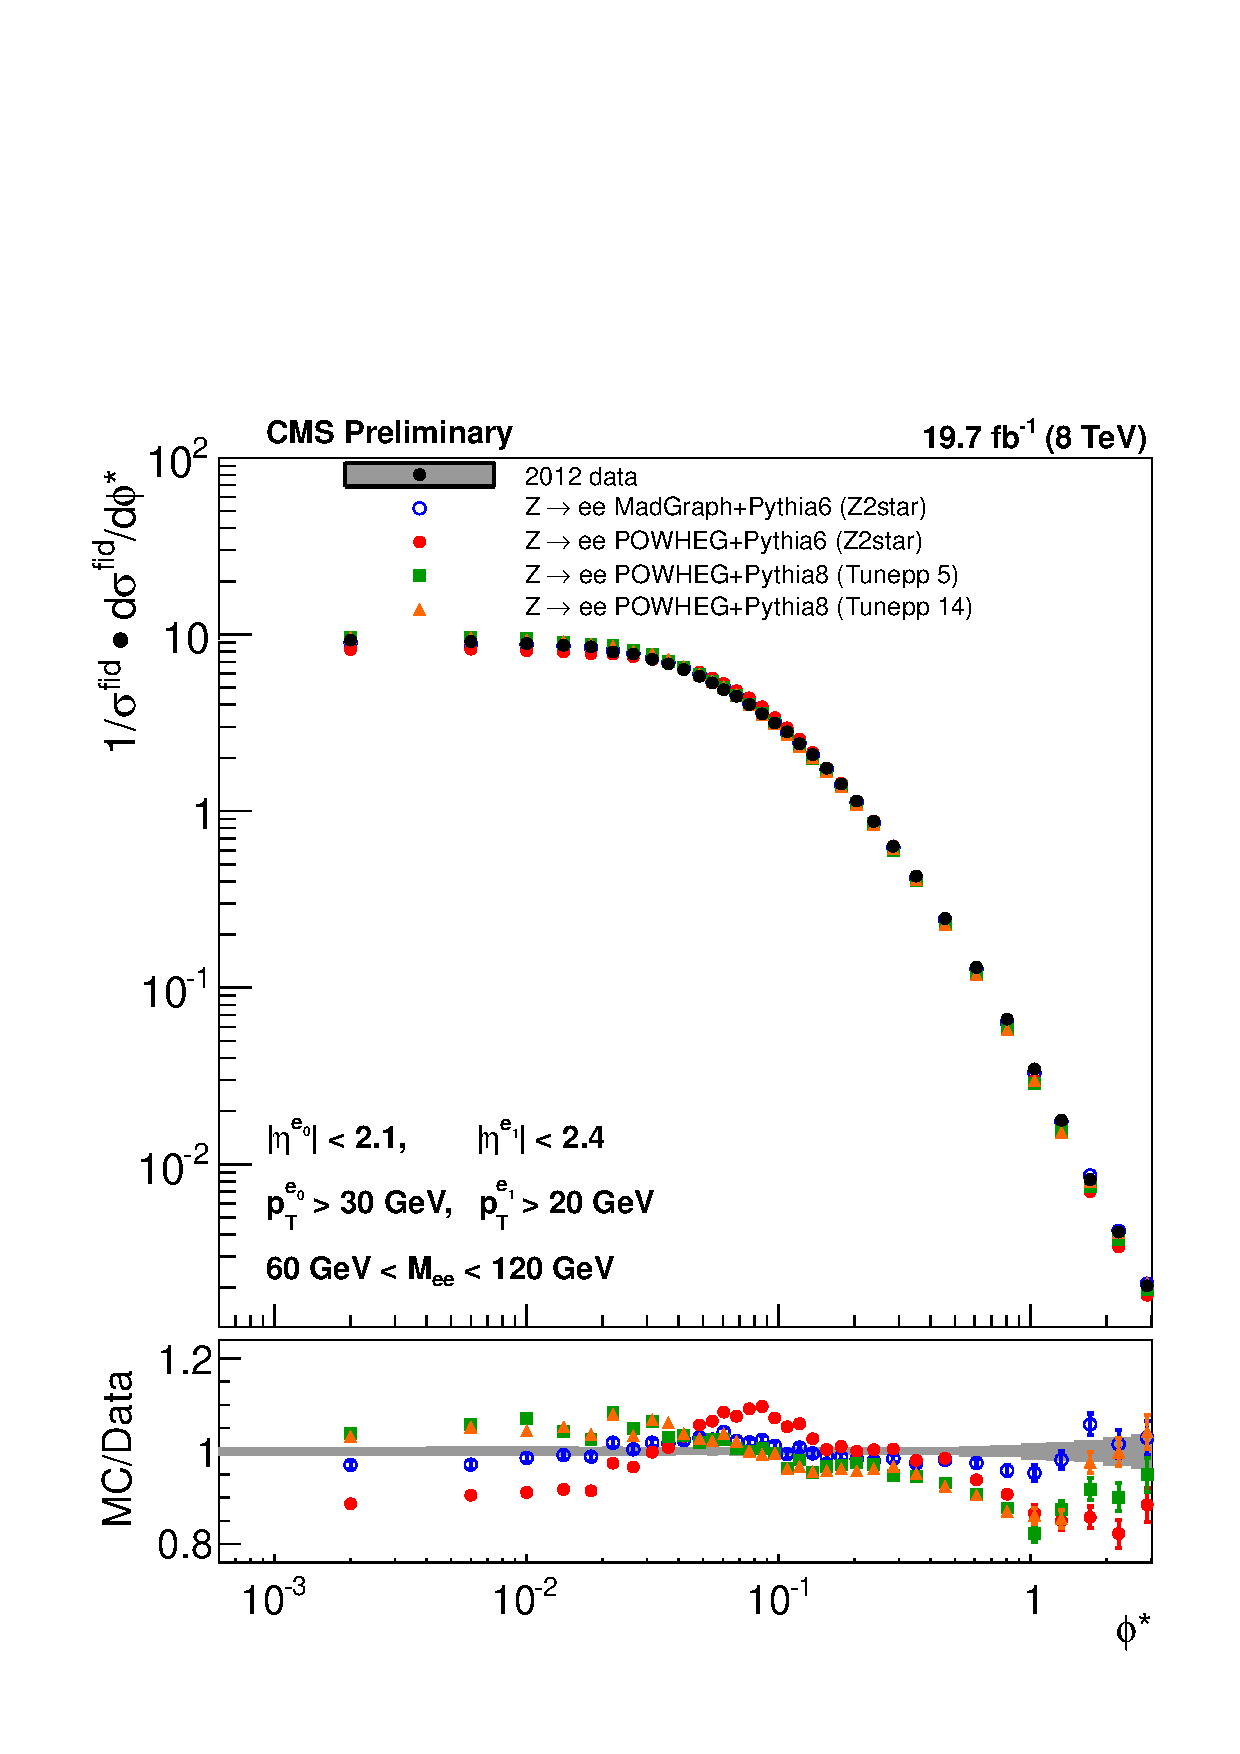
\includegraphics[width=\textwidth]{figures/ZShape_elec_PH_Norm_Dressed.pdf}
    \caption[
        The normalized differential cross section with respects to \phistar for
        \Ztoee events in our fiducial region from data unfolded with
        \PPsixZtwo.
    ]{
        The normalized differential cross section with respects to \phistar for
        \Ztoee events in our fiducial region from data unfolded with
        \PPsixZtwo, and the same distributions in \MADGRAPH and three versions
        of \POWHEG. A close up of the lower plot is shown in
        \cref{fig:results_ratio_norm_powheg}.
    }
    \label{fig:results_norm_powheg}
\end{figure}

\begin{figure}[!p]
    \centering
    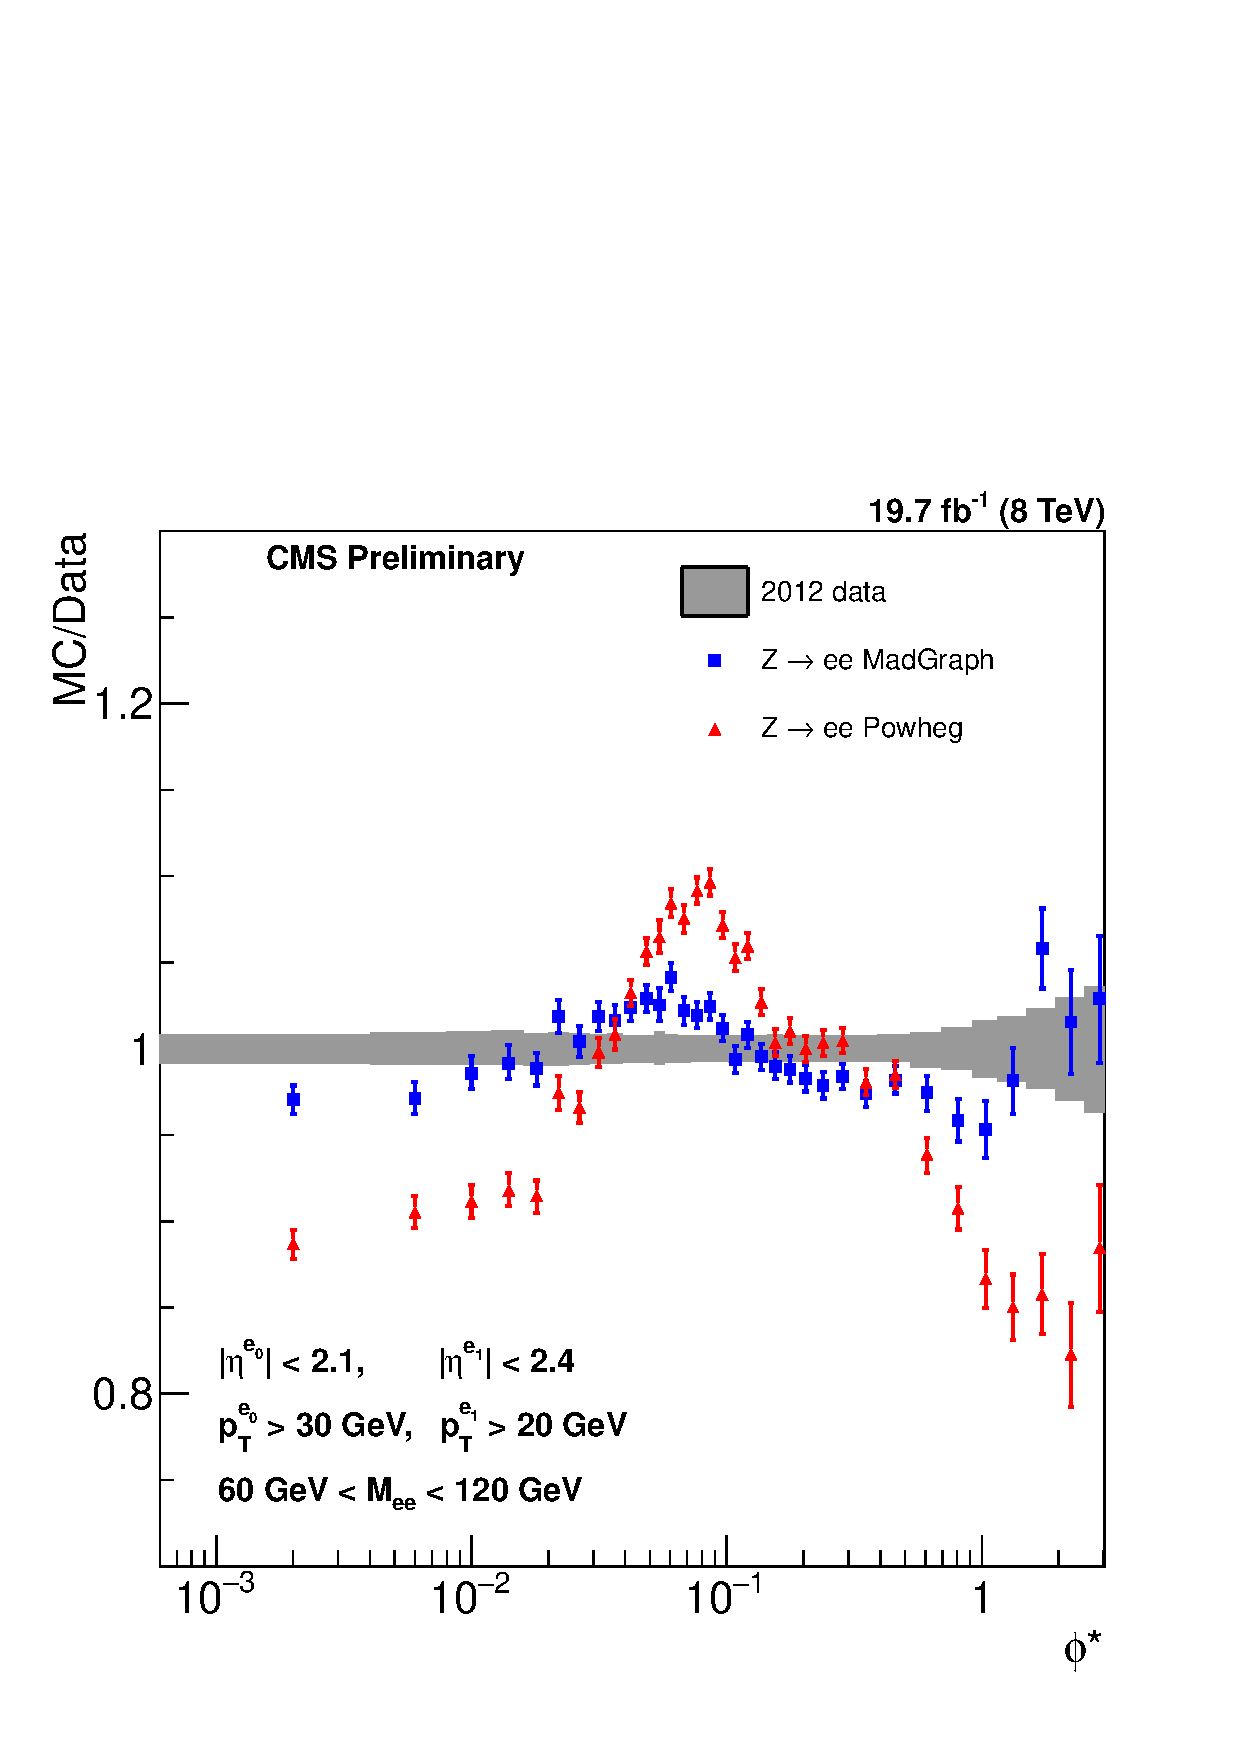
\includegraphics[width=\textwidth]{figures/ZShape_Ratioelec_PH_Norm_Dressed.pdf}
    \caption[
        Close up of the ratio plot from \cref{fig:results_norm} for the
        normalized cross section measurement unfolded with \PPsixZtwo.
    ]{
        Close up of the ratio plot from \cref{fig:results_norm} for the
        normalized cross section measurement unfolded with \PPsixZtwo. The
        error band indicates the uncertainty in the data, while the open
        circles show the ratio of \MADGRAPH over data, the filled circles show
        the ratio of \PPsixZtwo over data, the filled squares show the ratio of
        \PPeightTTfive over data, and the filled triangles show the ratio of
        \PPeightTTfourteen.
    }
    \label{fig:results_ratio_norm_powheg}
\end{figure}
